\chapter{Results}\label{ch:results}
All three selected models were tested on the 7,600 official test articles (1,900 per topic). For clean-trained \textit{Word TF-IDF LR}, we report its single deterministic score, while all augmented and neural conditions report three-seed means (seeds 42, 43, and 44). Single-seed checks are labeled explicitly.

\section{Spelling sensitivity}\label{sec:swap-sensitivity}
Under clean training, test accuracy drops steadily for every model as the swap target rises from 0\% to 20\%, though the size of the drop differs sharply across models (Figure~\ref{fig:core-robustness} and Table~\ref{tab:corefull}). The linear baseline (\textit{Word TF-IDF LR}) starts highest at $90.05\%$ and loses only $0.91$ percentage points across the sweep ($89.14\%$ at 20\% swaps), finishing more than $3.8$ percentage points ahead of both CNNs. \textit{Word CNN} takes the steepest hit, falling by $2.31$ percentage points from $86.79\%$ to $84.48\%$, while adding character fragments in \textit{Subword CNN} trims that drop to $1.86$ percentage points ($87.18\%$ to $85.32\%$). Across all three seeds on the original 20\% draw under augmented training, \textit{Subword CNN} beats \textit{Word CNN} by $+1.30$ percentage points ($85.77\%$ vs.\ $84.47\%$, 95\% bootstrap interval $[+0.95, +1.64]$, with the role of training schedule length examined in Section~\ref{sec:limitations} and Appendix~\ref{app:decisions}).

\begin{figure}[!htbp]\centering
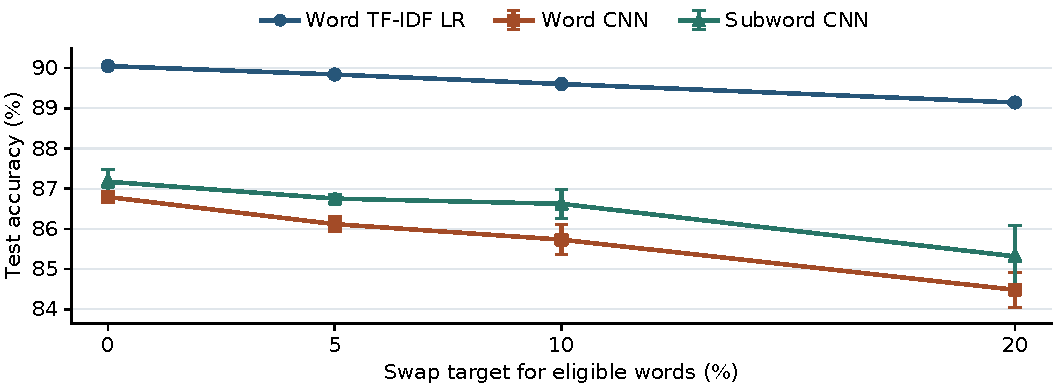
\includegraphics[width=.94\linewidth]{figures/core_robustness.pdf}
\caption[Accuracy across swap targets]{Official test accuracy (\%) across swap targets under clean training. CNN error bars indicate $\pm 1$ sample standard deviation across seeds 42, 43, and 44 (at 20\% swaps, $s = 0.43$ percentage points for \textit{Word CNN} and $s = 0.76$ for \textit{Subword CNN}).}\label{fig:core-robustness}
\end{figure}

\begin{table}[htbp]\centering\small
\begin{tabular}{llrrrr}\toprule
Model & Training arm & 0\% swaps & 5\% swaps & 10\% swaps & 20\% swaps \\\midrule
\textit{Word TF-IDF LR} & Clean & 90.05 / 90.03 & 89.84 / 89.82 & 89.61 / 89.59 & 89.14 / 89.12 \\
 & Augmented & 90.11 / 90.09 & 89.99 / 89.97 & 89.79 / 89.78 & 89.26 / 89.24 \\
\textit{Word CNN} & Clean & 86.79 / 86.79 & 86.12 / 86.10 & 85.73 / 85.71 & 84.48 / 84.46 \\
 & Augmented & 86.57 / 86.55 & 85.97 / 85.95 & 85.75 / 85.72 & 84.47 / 84.44 \\
\textit{Subword CNN} & Clean & 87.18 / 87.15 & 86.75 / 86.72 & 86.62 / 86.58 & 85.32 / 85.26 \\
 & Augmented & 87.32 / 87.29 & 87.02 / 86.99 & 86.72 / 86.69 & 85.77 / 85.73 \\\bottomrule
\end{tabular}
\caption[Official test results]{Official test accuracy / Macro-F1 (\%) across swap targets and training arms. Non-deterministic rows average seeds 42, 43, and 44, and seed standard deviations appear in Appendix~\ref{app:decisions}.}\label{tab:corefull}\end{table}

\section{Swap augmentation}
Next, we check whether static swap augmentation helps models handle spelling noise without hurting clean accuracy. At the original 20\% swap target (seed 41001), augmentation helps \textit{Subword CNN} the most, raising its mean accuracy by $+0.46$ percentage points ($85.32\%$ to $85.77\%$, 95\% paired bootstrap interval $[+0.03, +0.90]$, Figure~\ref{fig:augmentation-review}). Still, results vary widely across fitting seeds: seed 42 gained $+1.08$ percentage points and seed 43 gained $+0.36$, while seed 44 fell slightly by $-0.07$.

\begin{figure}[htbp]\centering
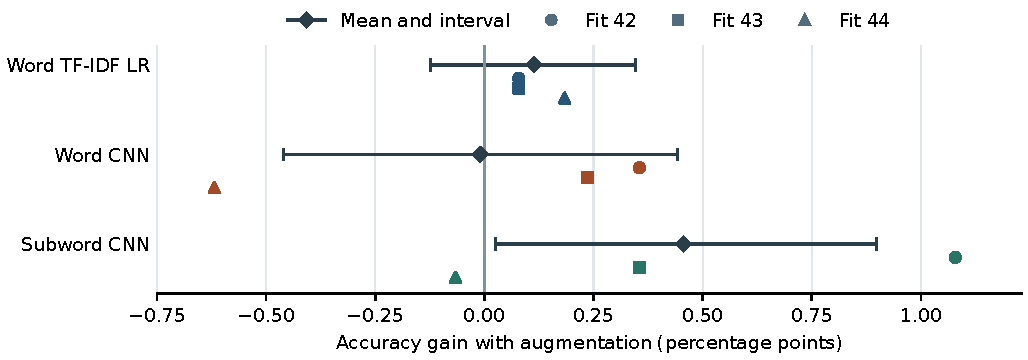
\includegraphics[width=.94\linewidth]{figures/augmentation_review.pdf}
\caption[Augmentation accuracy gains]{Accuracy differences (augmented minus clean, percentage points) at the original 20\% test swap target. Markers show seeds 42, 43, and 44, and diamonds mark three-seed means with pointwise 95\% paired bootstrap intervals.}\label{fig:augmentation-review}
\end{figure}

The other two models barely move with augmentation at 20\% swaps. \textit{Word TF-IDF LR} shifts by $+0.11$ percentage points ($89.14\%$ to $89.26\%$, 95\% interval $[-0.12, +0.35]$, alongside its validation-selected change from $C = 2.0$ to $C = 8.0$), and \textit{Word CNN} stays flat at $-0.01$ percentage points ($84.48\%$ to $84.47\%$, $[-0.46, +0.44]$). On clean test text ($0\%$ swaps), all three 95\% intervals cross zero ($+0.05$ for the baseline, $-0.22$ for \textit{Word CNN}, and $+0.14$ for \textit{Subword CNN}), showing no clear aggregate clean-text change.

\paragraph{Extra swap draws.}
Scoring all 18 saved checkpoints on two extra 20\% test swap draws (seeds 41002 and 41003) confirms that these rankings do not depend on one random set of word edits. \textit{Word TF-IDF LR} leads in every draw and arm, and each clean-trained model's three-seed mean varies by less than $0.45$ percentage points across draws. As Table~\ref{tab:augmentation-draws} shows, \textit{Subword CNN} keeps the largest mean augmentation gain ($+0.46$, $+0.39$, and $+0.31$ percentage points), while \textit{Word CNN} stays near zero and switches sign ($-0.01$, $+0.12$, and $-0.04$).

\begin{table}[!htbp]
\centering\small
\begin{tabular}{@{}lrrr@{}}
\toprule
Model & Original draw (41001) & Extra draw 1 (41002) & Extra draw 2 (41003) \\
\midrule
\textit{Word TF-IDF LR} & $+0.11$ & $+0.14$ & $+0.08$ \\
\textit{Word CNN} & $-0.01$ & $+0.12$ & $-0.04$ \\
\textit{Subword CNN} & $+0.46$ & $+0.39$ & $+0.31$ \\
\bottomrule
\end{tabular}
\caption[Gains across swap draws]{Mean augmentation accuracy gain (augmented minus clean, percentage points) across three independent 20\% test swap draws, averaging seeds 42, 43, and 44.}
\label{tab:augmentation-draws}
\end{table}
\FloatBarrier

The same seed pattern inside \textit{Subword CNN} shows up across all three draws (full per-seed numbers are in Appendix~\ref{app:decisions}). Seed 42 gains $+0.96$ to $+1.14$ percentage points across the draws, seed 43 gains $+0.36$ and $+0.37$ before tying at $0.00$ in the third draw, and seed 44 loses accuracy in every draw ($-0.07$, $-0.33$, and $-0.03$).

Even when aggregate scores look stable across swap draws, individual article predictions still shift from draw to draw. Across the three 20\% draws, fixed clean-trained checkpoints flipped correctness on $6.1\%$ of the 7,600 test articles for \textit{Word TF-IDF LR}, compared with $11.8\%$ for \textit{Word CNN} and $11.3\%$ for \textit{Subword CNN} (averaged across their three fits). Official test article 0, the Business pension story traced in Table~\ref{tab:article-trace}, is a clear example: clean-trained \textit{Subword CNN} (seed 42) misclassified it as World on the first two 20\% draws and predicted Business on the third, while the linear baseline predicted Business on all three.

\section{Confirmation check}
To verify that these findings hold outside the official test set used during early checks, we evaluated the frozen seed-42 checkpoints on the untouched 4,000-article confirmation split at 0\% and 10\% swaps (Table~\ref{tab:held-out-review}). The exact same ranking holds in every column: \textit{Word TF-IDF LR} leads, followed by \textit{Subword CNN} and then \textit{Word CNN}, with augmented \textit{Subword CNN} beating \textit{Word CNN} by $+1.30$ percentage points at 10\% swaps ($86.75\%$ vs.\ $85.45\%$). Inside \textit{Subword CNN}, augmentation raises 10\%-swap accuracy by $+0.60$ percentage points ($86.15\%$ to $86.75\%$) while lowering clean accuracy by $0.45$ points before rounding ($88.12\%$ to $87.68\%$), showing a small clean-text tradeoff on unseen articles.

\begin{table}[!htbp]\centering\small
\begin{tabular}{lrrrr}\toprule
 & \multicolumn{2}{c}{Clean training} & \multicolumn{2}{c}{Augmented training} \\
\cmidrule(lr){2-3}\cmidrule(lr){4-5}
Model & 0\% swaps & 10\% swaps & 0\% swaps & 10\% swaps \\\midrule
\textit{Word TF-IDF LR} & 90.50 & 89.70 & 90.12 & 89.65 \\
\textit{Word CNN} & 87.00 & 85.62 & 86.60 & 85.45 \\
\textit{Subword CNN} & 88.12 & 86.15 & 87.68 & 86.75 \\
\bottomrule
\end{tabular}
\caption[Confirmation set accuracy]{Classification accuracy (\%) on the untouched 4,000-article confirmation sample for frozen primary-run models at 0\% and 10\% swaps.}\label{tab:held-out-review}
\end{table}


\section{Error analysis}\label{sec:error-analysis}
Finally, we look beneath overall accuracy to see which topics suffer most from spelling swaps and how often individual articles flip between right and wrong predictions.

\subsection{Errors by topic}
Per-topic $F_1$ scores for clean-trained seed-42 models (Table~\ref{tab:topic-f1}) show large differences across categories. \emph{Sports} is the easiest topic for every model ($94.46\%$ $F_1$ for \textit{Word TF-IDF LR} and $90.75\%$ to $91.88\%$ for the CNNs at 20\% swaps), helped by distinctive team, league, and match names. \emph{Business} has the lowest $F_1$ across the board and suffers the largest 20\%-swap drops in the CNNs, falling by $3.49$ percentage points in \textit{Word CNN} ($83.07\%$ to $79.58\%$) and $4.09$ points in \textit{Subword CNN} ($83.07\%$ to $78.97\%$, before rounding). In \textit{Word TF-IDF LR}, \emph{Business} drops by only $0.85$ points ($86.37\%$ to $85.52\%$) and \emph{Sci/Tech} by $1.00$ point.

\begin{table}[htbp]\centering\small
\begin{tabular}{lrrrrrr}\toprule
 & \multicolumn{2}{c}{\textit{Word TF-IDF LR}} & \multicolumn{2}{c}{\textit{Word CNN}} & \multicolumn{2}{c}{\textit{Subword CNN}} \\
\cmidrule(lr){2-3}\cmidrule(lr){4-5}\cmidrule(lr){6-7}
Topic & 0\% & 20\% & 0\% & 20\% & 0\% & 20\% \\\midrule
World & 90.91 & 89.96 & 87.20 & 84.21 & 87.38 & 84.21 \\
Sports & 95.31 & 94.46 & 92.79 & 90.75 & 93.33 & 91.88 \\
Business & 86.37 & 85.52 & 83.07 & 79.58 & 83.07 & 78.97 \\
Sci/Tech & 87.54 & 86.53 & 84.46 & 82.76 & 84.64 & 82.48 \\
\bottomrule
\end{tabular}
\caption[Per-topic F1 scores]{$F_1$ scores by topic (\%) on the official test set for the models trained on clean text with seed 42 at the 0\% and 20\% swap targets.}\label{tab:topic-f1}
\end{table}


\FloatBarrier
Net changes in correctly classified articles per true topic from 0\% to 20\% swaps (Table~\ref{tab:topic-correct-change}) confirm that Business drives almost all of the neural accuracy loss. Out of 1,900 Business test articles, clean-trained seed-42 \textit{Word CNN} loses 172 net correct predictions (90.5\% of its 190 total net losses) and \textit{Subword CNN} loses 181 (90.0\% of 201), compared with just 28 for the linear baseline.

\begin{table}[!htbp]
\centering\small
\begin{tabular}{@{}lrrr@{}}
\toprule
True topic & \textit{Word TF-IDF LR} & \textit{Word CNN} & \textit{Subword CNN} \\
\midrule
World ($N = 1{,}900$) & $-11$ & $+28$ & $+31$ \\
Sports ($N = 1{,}900$) & $-16$ & $-61$ & $-50$ \\
Business ($N = 1{,}900$) & $-28$ & $-172$ & $-181$ \\
Sci/Tech ($N = 1{,}900$) & $-14$ & $+15$ & $-1$ \\
\midrule
Total net change ($N = 7{,}600$) & $-69$ & $-190$ & $-201$ \\
\bottomrule
\end{tabular}
\caption[Topic correctness changes]{Net change in correctly classified test articles from 0\% to 20\% swaps for clean-trained seed-42 models. Positive values denote higher recall after corruption.}
\label{tab:topic-correct-change}
\end{table}
\FloatBarrier

At the same time, both CNNs actually predict \emph{more} true World articles correctly at 20\% swaps ($+28$ and $+31$, Table~\ref{tab:topic-correct-change}) even as World $F_1$ drops by $2.98$ percentage points in \textit{Word CNN} and $3.17$ points in \textit{Subword CNN} (Table~\ref{tab:topic-f1}). When spelling swaps knock out specific cues in Business, Sports, and Sci/Tech, the CNNs fall back to World more often. In \textit{Subword CNN}, true World hits rise by 31 (1,641 to 1,672), raising recall, while false-positive World predictions surge by 184 (215 to 399), pulling precision and $F_1$ sharply down.

In the clean-trained seed-42 \textit{Subword CNN} confusion matrix at 20\% swaps (Table~\ref{tab:confusion-review}), the biggest error counts are 320 true Business articles labeled as Sci/Tech (up from 239 on clean text) and 187 labeled as World (up from 92). These are mostly stories about technology companies or international economic policy where key financial terms were corrupted.

\begin{table}[!htbp]\centering\small
\begin{tabular}{lrrrr}\toprule
True topic & World & Sports & Business & Sci/Tech \\\midrule
World & \textbf{1,672} & 79 & 54 & 95 \\
Sports & 102 & \textbf{1,742} & 13 & 43 \\
Business & 187 & 41 & \textbf{1,352} & 320 \\
Sci/Tech & 110 & 30 & 105 & \textbf{1,655} \\
\bottomrule
\end{tabular}
\caption[Confusion matrix for Subword CNN trained on clean text at 20\% swaps]{Confusion matrix on the official test set at the 20\% swap target for Subword CNN trained on clean text (seed 42). Rows correspond to true topics (1,900 articles per row) and columns correspond to predicted topics. Diagonal entries in bold indicate correct classifications.}\label{tab:confusion-review}
\end{table}


\FloatBarrier
Four test articles scored by clean-trained \textit{Subword CNN} (seed 42) at 20\% swaps show how single word swaps trigger new errors or accidental fixes:

\paragraph{Australian insurer.}
In a story on an Australian insurance group returning to profit after British losses, swapping \texttt{insurer} $\to$ \texttt{inusrer}, \texttt{disastrous} $\to$ \texttt{disasrtous}, and \texttt{pushed} $\to$ \texttt{pusehd} weakens financial cues while leaving \texttt{australian} and \texttt{britain} intact, shifting the prediction from Business to World.

\paragraph{Malpractice protest.}
A report on doctors suspending elective surgeries over rising malpractice insurance rates flips from Business to World when \texttt{surgeries} becomes \texttt{surgreies}, changing a window activation in a story blending medicine and insurance economics.

\paragraph{Mobile wiretaps.}
Coverage of a law-enforcement wiretap request on push-to-talk phones shifts from Sci/Tech to World after \texttt{push} becomes \texttt{psuh}, weakening the telecom cue relative to federal regulatory wording.

\paragraph{Honda racing bid.}
A story on Honda's bid for a Formula One racing team was misclassified as Sci/Tech on clean text because of automotive words, and corrupting \texttt{partner} $\to$ \texttt{parnter} lowers the competing Sci/Tech score enough to recover Sports.

\subsection{Prediction churn}
On the 10\%-swap validation view, out-of-vocabulary token rates in \textit{Word CNN}'s 30,000-entry vocabulary jump fourfold from roughly $2\%$ on clean text to $8\%$ under clean training, compared with $3\%$ to $5\%$ under augmented training (where training typos enter the vocabulary). Yet, as the Honda example shows, losing a word cue can also hide a misleading feature and fix a prior mistake. Figure~\ref{fig:paired-changes} pairs clean-trained seed-42 predictions across all 7,600 official test articles against their 5\%, 10\%, and 20\% swap versions.

\begin{figure}[!htbp]
\centering
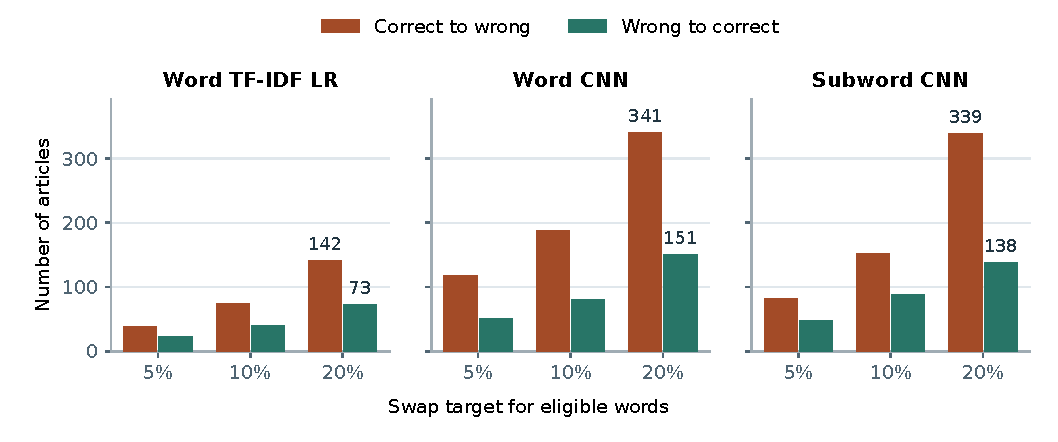
\includegraphics[width=.82\linewidth]{figures/paired_prediction_changes.pdf}
\caption[Paired prediction flips]{Paired prediction changes across the 7,600 official test articles for clean-trained seed-42 models relative to 0\% swaps (brown indicates new errors and green indicates corrected errors).}
\label{fig:paired-changes}
\end{figure}

At 20\% swaps, \textit{Word TF-IDF LR} makes 142 new errors (clean correct $\to$ swap wrong) while fixing 73 prior clean-text mistakes (clean wrong $\to$ swap correct). That net loss of $142 - 73 = 69$ articles ($-0.91$ percentage points) hides $142 + 73 = 215$ flipped predictions. Both CNNs show more than twice as much churn: \textit{Word CNN} (seed 42) makes 341 new errors and 151 fixes (net $-190$ articles, 492 flips), and \textit{Subword CNN} (seed 42) makes 339 new errors and 138 fixes (net $-201$ articles, 477 flips).

At seed 42, \textit{Subword CNN} makes fewer new errors than \textit{Word CNN} at 5\% (82 vs.\ 118) and 10\% swaps (153 vs.\ 188), but at 20\% swaps their new errors converge (339 vs.\ 341). Because \textit{Word CNN} records 13 more accidental fixes (151 vs.\ 138), its single-seed net drop is slightly smaller ($2.50$ vs.\ $2.64$ percentage points), which underlines why the multi-seed comparison in Section~\ref{sec:swap-sensitivity} matters.
